\chapter{Next plans}

\label{Work_Plan}


\section{Active learning for a surrogate}
In high dimensions, the number of data points required for \textit{experiment of design} based on \textit{Monte Carlo} for a surrogate can be prohibitive as the computational cost is too expensive. Active learning provides as a tool to explore the random space in a sequential and, therefore, affordable way. They are built adaptively in an attempt to finely approximate the limit-state surface in areas of high probability mass. Next, we hope to identify new sampling locations by minimizing an acquisition function based on a \acrshort{PCE} model.





\section{A unified and scalable digital twin for piles}

\subsubsection{Urgent need for a unified and scalable digital twin}

To address these challenges in real time, digital twin (DT) has gained popularity in handling abundant data and predict the pile's response in a more organized and accurate manner \citep{wang2021}. DT can effectively leverage various data sources, including physical models, sensor updates and operating history. They seamlessly integrate simulation processes to dynamically replicate the behavior of a physical system in a virtual space in real-time. 


 However, in a context of geotechnical engineering problem, while the value proposition of digital twin has become widely appreciated, the pile design process remains in a custom production phase. Current digital twin for offshore piles are still bespoken, relying on highly specialized implementations and thus requiring considerable resources and expertise to deploy and maintain. Therefore, it is necessary to move toward digital twins at scale by developing a rigorous and unified mathematical foundation. 


\subsubsection{Benefits of \acrlong{POPGM}}



Introducing probabilistic graphical model (\acrshort{PGM}) involving in Bayesian inverse analysis can visualize the calculation and combine decision theory naturally to make prompt predictions. Besides, as a mathematical and rigorous foundation, \acrshort{PGM} is proposed to support the transition from custom defined model towards accessible digital twins at scale. Based on such flexible asset-specific models, the entire loading life-cycle can be incorporated into a digital twin forming a unified and accessible foundation for a wide range of offshore piles. Combined with monitored data, the proposed dynamic updated digital twin can be very important to provide rapid analysis results for reliable soil parameters and enables intelligent decision making on the pile behaviors. 

 Followed by \cite{kapteyn2021}, we can introduce \textit{Rewards} and \textit{Actions}. \acrfull{POPGM} can be implemented in our own setting in \cref{fig: POMDP}. This process can be roughly divided into two main parts: (1) calibration and assimilation; (2) prediction; as shown in \cref{eq: DA_predict} and \cref{eq: DA_assimilation}, respectively:
\begin{figure}[htbp]
    \centering
    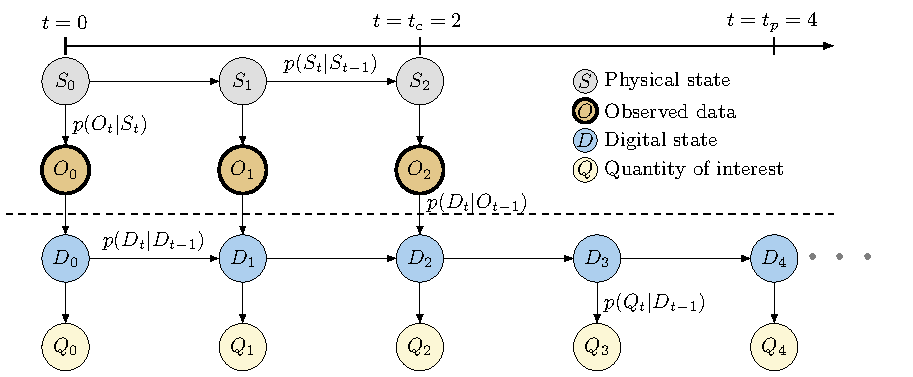
\includegraphics[width = 190mm]{Figures/figure-POMDP.pdf}
 \caption{\acrshort{POPGM} in digital twin}
 \label{fig: POMDP}
\end{figure}
\begin{equation}
\begin{aligned}
& p(D_{0},...,D_{t_{c}},Q_{0},...,Q_{t_{c}},R_{0},...,R_{t_{c}}|o_{0},...,o_{t_{c}},u_{0},...,u_{t_{c}}) \\
& = \prod_{t=0}^{t_{c}}[\phi_{t}^{update}\phi_{t}^{QoI}\phi_{t}^{evaluation}] \label{eq: DA_predict}
\end{aligned}
\end{equation}
\begin{equation}
\begin{aligned}
    & p(D_{0},...,D_{t_{p}},Q_{0},...,Q_{t_{p}},R_{0},...,R_{t_{p}},U_{t_{c}+1},...,U_{t_{p}}|o_{0},...,o_{t_{c}},u_{0},...,u_{t_{c}}) \\
    & \propto \prod_{t=0}^{t_{p}}[\phi_{t}^{dynamics}\phi_{t}^{QoI}\phi_{t}^{evaluation}] \prod_{t=0}^{t_{c}}\phi_{t}^{assimilation} \prod_{t=t_{c}+1}^{t_{p}}\phi_{t}^{control} \label{eq: DA_assimilation}
\end{aligned}
\end{equation}


\section{Next implementation for a pile:}


\subsubsection{Stage 1}
Calibrate the models in \cref{fig: CM2pile} with \acrshort{POPGM} shown in \cref{fig: POMDP}.
\begin{figure}[H]
    \centering
    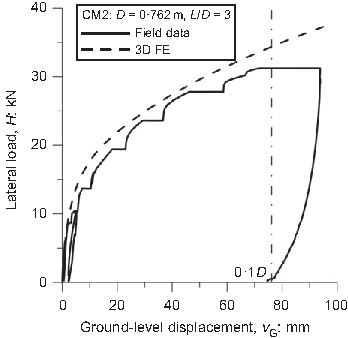
\includegraphics[width = 90mm]{Figures/figure-CM2.pdf}
\caption{CM2 pile load displacement from \protect\cite{zdravkovic2020}}
\label{fig: CM2pile}
\end{figure}
Computational forward model settings are listed:
\begin{itemize}[left=0cm]
    \item Software: $\href{https://www.imperial.ac.uk/geotechnics/research/facilities-and-expertise/icfep/}{\rm{Imperial \ College \ Finite\ Element\ Program}}$ (details can be seen in the link).
    \item Constitutive model: clay model adapted from \cite{zdravkovic2020} and sand model adapted from \cite{taborda2020}.
\end{itemize}
Objective: Ensure the soil parameters in digital model can reveal unique characteristics of piles.

\subsubsection{Stage 2}
In operational phase, based on \acrshort{POPGM} in \cref{fig: POMDP}, continue the assimilation process: extend the digital twin capability to capture the piles response during loading.

\subsubsection{Stage 3}
Extension to prediction on the predictive pile performance. 



\section{Time plan}
\begin{table}[H]
\caption{PhD timeline}
\label{table: work_plan}
\vspace{10pt}
\centering
\resizebox{\textwidth}{!}{
\begin{tabular}{|l|l|l|l|l|l|l|l|l|l|l|l|l|l|l|l|l|l|}
\hline
month                                                                           & 0 & 3                     & 6 & 9 & 12 & 15 & 18 & 21 & 24 & 27 & 30 & 33 & 36 & 39 & 42 & 45 & 48 \\ \hline
Literature review                                                               & \checkmark &\checkmark               &\checkmark   &   &    &    &    &    &    &    &    &    &    &    &    &    &    \\ \hline
\begin{tabular}[c]{@{}l@{}}Numerical modelling\\ (Data collection)\end{tabular} &   &\checkmark&  \checkmark & \checkmark  & \checkmark   &\checkmark    & \checkmark   &    &    &    &    &    &    &    &    &    &    \\ \hline
\begin{tabular}[c]{@{}l@{}}Statistics Methods \\ learning\end{tabular}          &   &\checkmark                       &\checkmark   & \checkmark  &\checkmark    & \checkmark   &   \checkmark &\checkmark    &\checkmark    &    &    &    &    &    &    &    &    \\ \hline
\begin{tabular}[c]{@{}l@{}}Statistics analysis\\ calibration\end{tabular}       &   &                       & \checkmark  &  \checkmark & \checkmark   &    &    &    &    &    &    &    &    &    &    &    &    \\ \hline
\begin{tabular}[c]{@{}l@{}}Statistics analysis\\ assimilation\end{tabular}      &   &                       &   &   &    &  \checkmark  &   \checkmark &\checkmark    &  \checkmark  & \checkmark   &\checkmark    &    &    &    &    &    &    \\ \hline
\begin{tabular}[c]{@{}l@{}}Statistics analysis\\ prediction\end{tabular}        &   &                       &   &   &    &    &    &    &    &    &   &  \checkmark  &   \checkmark &  \checkmark   &    &    &    \\ \hline
Thesis writing                                                                  &   &                       &   &   &    &    &    &    &    &    &    &    &    &    &     \checkmark&  \checkmark   & \checkmark    \\ \hline
Journal/Conference                                                              &   &                       &   &   &    &    &    &     \checkmark&    &    &    &    \checkmark &    &    &    &    &  \checkmark   \\ \hline
\end{tabular}}
\end{table}
